\chapter{Analysis}
\label{ch:4}

This chapter analyzes the problem of the retail site selection process from the user's point of view, examining it from various angles to understand the challenges and requirements associated with choosing an optimal location. The examination unfolds in three sections: an understanding of the use cases, a technical analysis, and a review of existing tools.

\section{Target Audience}
\label{section:target-audience}

The primary beneficiaries of this system are non-professional individuals, such as aspiring entrepreneurs, small business owners, or local retailers seeking to expand. These individuals often lack technical expertise in geographic analysis but require informed decisions for choosing the right location for their new outlet.

\section{Use Cases}

In the dynamic world of retail, major players and emerging businesses alike recognize the critical importance of strategic location decisions. Large retail stores or newcomers often use the assistance of specialized experts. Hiring specialists for the retail site decision process involves professionals with backgrounds in market analysis, real estate, and business development. These experts leverage their experience to conduct thorough assessments, providing valuable insights that inform decision-making. 

While the expertise of specialists enhances the strategies of larger retailers, the reality is that many small retailers face financial constraints that may limit their ability to use such assistance. Recognizing the unique challenges of resource limitations, small retailers can explore alternative solutions, such as systems, to overcome the challenges of opening new locations.

The most general cases in which such a system could help are, for example, identifying high-potential areas, competitive analysis and location evaluation.

\subsection{Identifying High-Potential Areas}
\label{analysis:high-potential-areas}

Identifying high-potential areas for opening new retail outlets is a crucial step in strategic business. This process involves a comprehensive analysis of various demographic factors to pinpoint locations where a retail establishment is likely to thrive. The goal is to maximize the chances of success by aligning the business with the preferences, needs, and behaviours of the target market in a specific geographical area. 

To identify high-potential areas, certain requirements must be met. Firstly, there should be the availability of comprehensive data sets pertaining to demographics and consumer behaviour. Access to reliable and up-to-date data sources is crucial as it ensures the accuracy of the analysis.

In addition, implementing advanced analytical tools becomes essential. These tools are necessary for processing and interpreting the vast amount of data involved in the identification process. Geographic Information System (GIS) tools and data visualization platforms play a significant role in contributing to effective decision-making in this context.

\subsection{Competitive Analysis}

Competitive analysis is a systematic process of understanding the competitive landscape within a particular industry. It involves the examination of key players and their strengths and weaknesses. The primary objective is to gain insights to inform strategic decision-making, enabling businesses to position themselves effectively in the market.

For those without a background in market analysis, understanding the competitive landscape can be challenging. In this case, requirements stated in section \ref{analysis:high-potential-areas} are still relevant. Moreover, the system should include data layering, similar to GIS, for displaying different data types.

\subsection{Location Evaluation}

Location evaluation involves analysis of potential locations to determine their suitability for establishing a new retail presence. This multifaceted assessment considers a range of factors that impact the success and viability of a retail operation in a specific geographic area.

Location evaluation poses a significant challenge for retailers because of the location attributes that are usually evaluated individually.

\section{Functional Requirements}

After examining the presented use case examples, I have identified essential functional requirements crucial for developing an effective tool for non-professional users.

\subsection{User Interface}

The system needs a user-friendly interface to cater to non-professional individuals seeking to expand their retail presence. This includes easy navigation through analytical tools and data visualizations without nesting them.

The user interface (UI) is a critical component of the location evaluation system, especially considering the non-professional individuals as the primary users. The UI should prioritize simplicity and intuitiveness to ensure accessibility for users without technical expertise in geographic analysis. A clean and well-organized design is essential, allowing users to navigate seamlessly through various analytical tools and features. Clear and concise menu structures, accompanied by easily understandable icons, should guide users through the process of identifying high-potential areas, conducting competitive analysis, and evaluating potential locations.

Visual elements within the UI, such as maps, should be presented in a way that facilitates easy interpretation of geographic data. The system should provide interactive elements, enabling users to manipulate and explore data effortlessly.

The UI should include contextual help features and tooltips to provide guidance throughout the analysis. Additionally, the system should offer user-friendly wizards or step-by-step workflows to assist users in conducting location evaluations.

\subsection{Data Integration}
\label{subsec:dataIntegration}

The system should provide an integration of custom datasets and their configuration. Different sources may provide information in diverse structures; for this reason, compatibility with various data formats is essential. The system is going to have a clearly defined format for datasets.

Data layering is a feature within the system that allows users to gain an understanding of the complex and interconnected factors.

The system should allow users to overlay different datasets onto a single map, creating informative layers that provide a comprehensive view of relevant information, similar to GIS data layering. For instance, users may overlay competitor locations and demographic data on the same map.

\section{Available Data}

The thesis relied on the data repository \texttt{data.brno}\footnote{Data of Brno---\url{https://data.brno.cz/}}, a platform that hosts numerous datasets released under open licenses\footnote{License for the datasets---\url{https://creativecommons.org/licenses/by/4.0/}}. Some of these datasets contain information crucial to the employed methodology. Understanding its contents is vital as subsequent chapters build upon this foundation. 

Additionally, I will use this portal's datasets to test and demonstrate the system, but in this section, I will only analyze relevant datasets and their structure. Their application I will describe in section \ref{sec:testingApplicationWithRealData}.

\subsection{Data Requirements}
\label{subsec:dataRequirements}

As was noted in the section \ref{sec:identifyingGeocompetition}, the system will use the Huff model, described in section \ref{section:huff-model}. This model requires such variables as the distance from a customer to a competitor and the size of a competitor. The distance can be calculated if the locations of a customer and a competitor are known.

The datasets that can fulfil these requirements for the system are ``Number of people living at the addresses`` and ``Brno retail research``. Both datasets follow the same initial data model, but they both differ in the ``properties`` attribute:

\begin{itemize}
    \item \textbf{features}---an array containing individual features.
    \begin{itemize}
        \item \textbf{type}---specifies the type of an object. In the case of these datasets, it is always set to ``feature``.
        \item \textbf{properties}---key-value pairs containing descriptive information about the feature.
        \item \textbf{geometry}---specifies the geometric shape of the feature.
        \begin{itemize}
            \item \textbf{type}---specifies the type of an object. In this model, it is always a ``Point`` geometry.
            \item \textbf{coordinates}---array with the longitude and latitude of the feature.
        \end{itemize}
    \end{itemize}
\end{itemize}

\subsection{Number of People Living at the Addresses}

The first dataset\footnote{Dataset with a number of people living at the addresses---\url{https://arcg.is/1Lfbzb0}} contains information on the number of people living at the addresses. It has the following model:

\begin{itemize}
    \item \textbf{pocet}---number of people
    \item \textbf{cislo\_dom}---house number
    \item \textbf{cislo\_ori\_zn}---reference number and symbol
    \item \textbf{ulice}---street name
\end{itemize}

Here is an example of this dataset (Listing \ref{lst:numberOfPeopleJson}):
\begin{lstlisting}[caption={Example of a ``Number of People Living at the Addresses`` dataset.}, label=lst:numberOfPeopleJson]
{
    "features": [
        { 
            "type": "Feature", 
            "properties": { 
                "objectid": 1, 
                "pocet": 4, 
                ...
            }, 
            "geometry": { 
                "type": "Point", 
                "coordinates": [ 16.58..., 49.17... ] 
            } 
        },
        ...
    ]
}
\end{lstlisting}

The only properties that are interesting to us are coordinates, latitude, and longitude, which represent the location of a potential customer, which is required in order to calculate the distance between a customer and a competitor.

\subsection{Brno Retail Research}

The second dataset\footnote{Brno retail research---\url{https://arcg.is/0CaaCS}} contains information about all the business outlets in Brno, such as area, type and many other less relevant attributes. The dataset has the following model:

\begin{itemize}
    \item \textbf{sluzba\_typ}---type of service
    \item \textbf{plocha}---size of retail outlet (area)
\end{itemize}

Here is an example of this dataset (Listing \ref{lst:brnoRetailResearchJson}):

\begin{lstlisting}[caption={Example of a ``Brno Retail Research`` dataset.}, label=lst:brnoRetailResearchJson]
{
    "features": [
        {
            "type": "Feature",
            "properties": {
                "sluzba_typ": "POH - restaurace",
                "plocha": "do 20",
                ...
            },
            "geometry": {
                "type": "Point",
                "coordinates": [ 16.58..., 49.17... ] 
            }
        },
        ...
    ]
}
\end{lstlisting}

Important properties in this dataset are the coordinates, ``plocha`` and ``sluzba\_typ``. Plocha represents the area of the outlet, while sluzba\_typ defines a category of a business. It will become more important further in the thesis.

\section{Existing Tools}
\label{analysis:existing-tools}

This section briefly explores existing solutions to the retail site selection problem for users seeking alternative ways to assist in a decision-making process. 

Selecting the best retail site involves a combination of market research, data analysis, and location scouting. There isn't a single software or web application that can make this decision for the retailer. However, there are software applications that can provide a user with a set of tools to help with decision-making, such as analyzing market share and competition, targeting new customers or determining new sites. The most recent approaches to solving the retail site selection problem involve GIS.

\subsection{Geographic Information System}

\begin{figure*}[ht]\centering
  \centering
  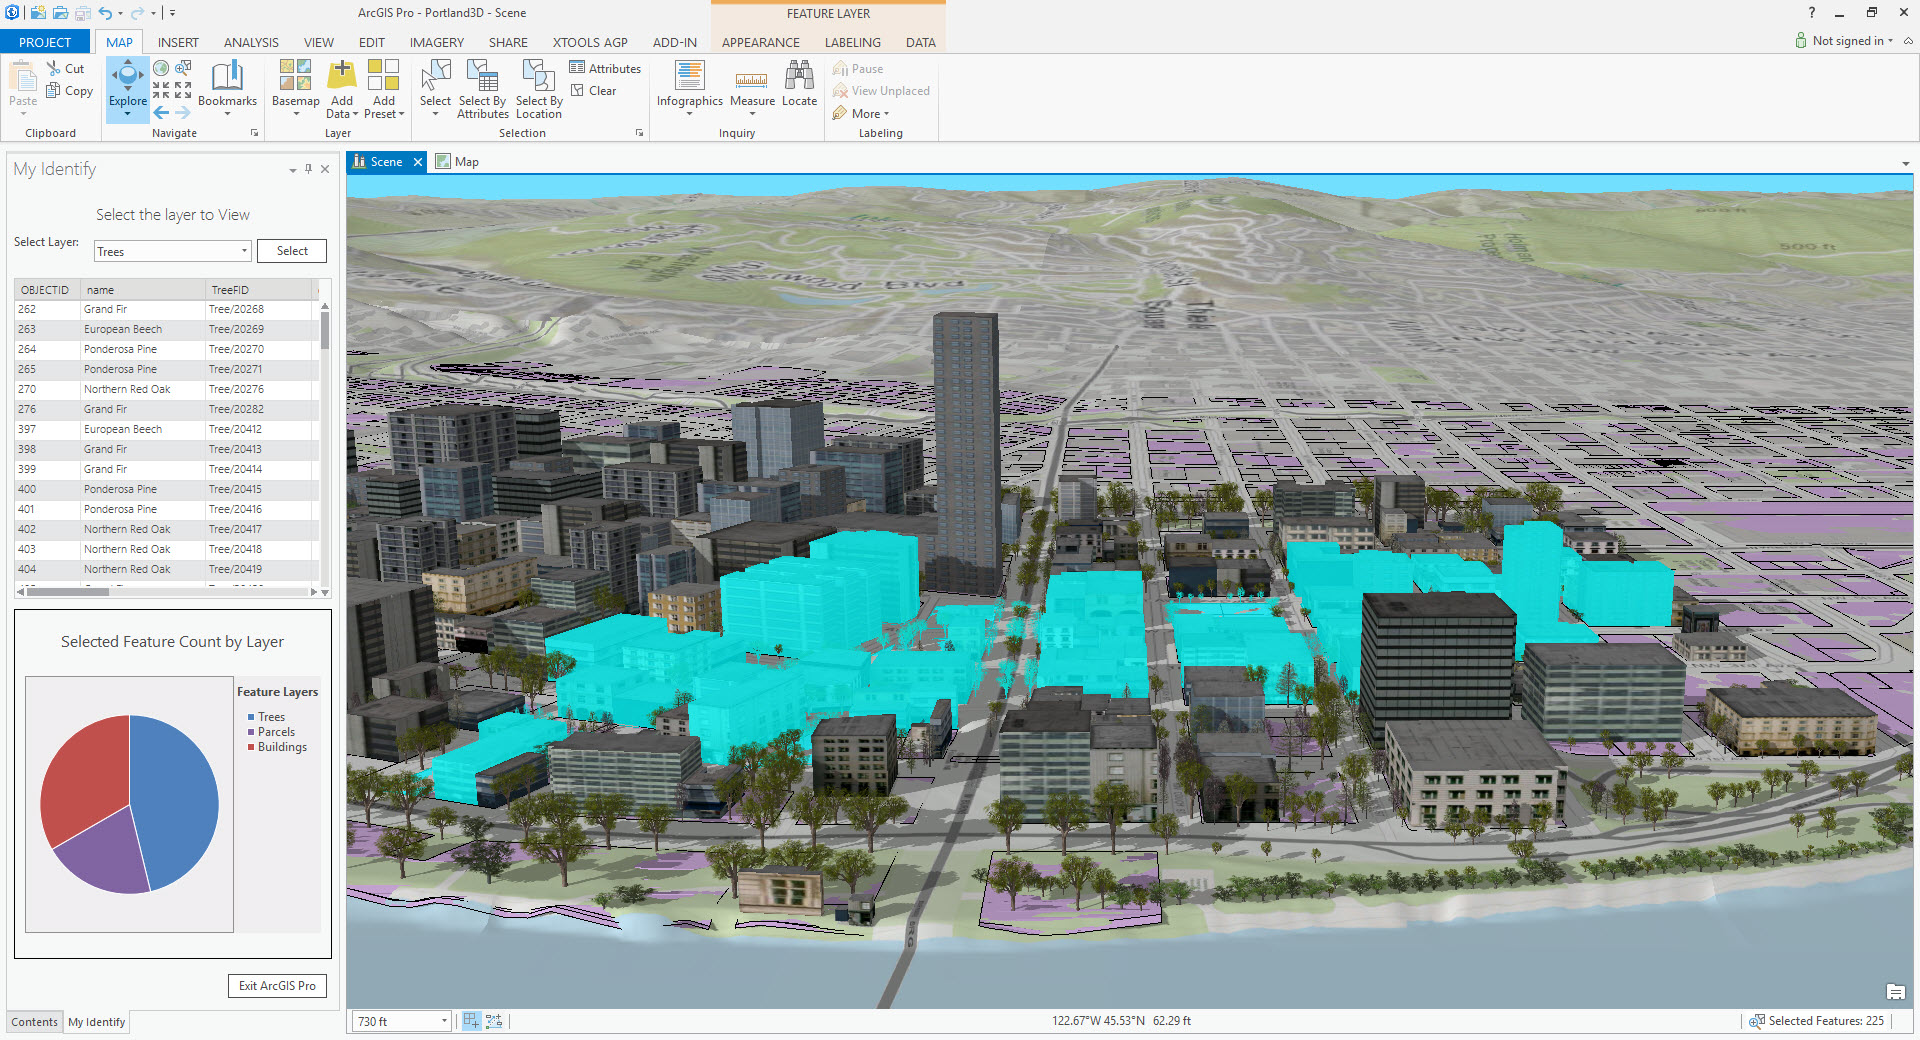
\includegraphics[width=0.75\linewidth]{obrazky-figures/ch4/arcgis-pro-3d.jpg}
  \caption{ArcGIS user interface}
  \label{fig:arc-gis}
\end{figure*}

As it was mentioned in Chapter \ref{ch:3}, geographic information systems are very powerful tools for spatial analysis, which provide the functionality to capture, store, query, analyze, display and output geographic information (Figure \ref{fig:arc-gis}). However, in order to conduct analysis related to retail site selection, these systems are used in conjunction with other tools and methods such as \textit{decision-making system} (DSS) and \textit{multi-criteria decision-making} (MCDM). These methods are not considered to be a part of GIS, but very often, they are provided as a separate set of extra tools to work with spatial data, and the user must know how to use them correctly.

There are also private GIS systems, such as Buxton. They offer a distinct advantage in accessing extensive datasets for comprehensive spatial analysis. Unlike publicly available GIS tools, these private systems often provide proprietary data sources, enabling users to delve deeper into layers of information.

\section{Conclusion}

As it was mentioned in the section \ref{analysis:existing-tools}, there isn't a single software or web application that can make decisions for the retailer because the process involves analysis of multiple variables that can have a simultaneous impact on the success of a business. For this reason, site selection is a complex problem that can be tackled using multiple models, methods and procedures, making the process even harder for those who are unaware of them, which is why not anyone can dive straight into GIS. Additionally, the entire decision process may include extra tools that are not directly related to GIS and may not be available in the same application.

From the analysis, it can be seen that most of the requirements are not met by existing solutions. Therefore, it is needed to build a custom one. Such a system should prioritize user-friendly interface and data integration. It should follow a specific procedure, which can also be configurable for an individual's needs. 

Creating a system that connects complex analytics with the needs of regular retailers is crucial for making retail decisions easier and available to everyone.